\documentclass[11pt,letterpaper]{article}

% --- Packages ---
\usepackage[utf8]{inputenc}
\usepackage[T1]{fontenc}
\usepackage{amsmath,amssymb,amsthm}
\usepackage{algorithm}
\usepackage{algpseudocode}
\usepackage{graphicx}
\usepackage{tikz}
\usetikzlibrary{shapes,arrows,positioning,calc,fit,decorations.pathreplacing}
\usepackage{listings}
\usepackage{xcolor}
\usepackage{hyperref}
\usepackage{geometry}
\usepackage{booktabs}
\usepackage{enumitem}
\usepackage{caption}
\usepackage{subcaption}

\geometry{margin=1in}

% --- Code listing style ---
\definecolor{codebg}{rgb}{0.95,0.95,0.95}
\definecolor{codegreen}{rgb}{0.0,0.5,0.0}
\definecolor{codegray}{rgb}{0.5,0.5,0.5}
\definecolor{codepurple}{rgb}{0.58,0,0.82}

\lstset{
    backgroundcolor=\color{codebg},
    basicstyle=\ttfamily\footnotesize,
    keywordstyle=\color{codepurple}\bfseries,
    commentstyle=\color{codegreen},
    stringstyle=\color{red},
    numbers=left,
    numberstyle=\tiny\color{codegray},
    numbersep=5pt,
    breaklines=true,
    frame=single,
    rulecolor=\color{codegray},
    tabsize=4
}

% --- Theorem environments (CLRS-style) ---
\theoremstyle{definition}
\newtheorem{definition}{Definition}[section]
\newtheorem{theorem}{Theorem}[section]
\newtheorem{lemma}[theorem]{Lemma}
\newtheorem{invariant}{Invariant}[section]

% --- Title ---
\title{\textbf{sotOS: A Capability-Based Microkernel with Per-Core IPC,\\
WASM Software Fault Isolation, and Formal Verification}\\[0.5em]
\large Technical Report}

\author{Santiago Sotomonte\\
\texttt{sotOS Project}}

\date{March 2026}

\begin{document}
\maketitle

\begin{abstract}
We present \textbf{sotOS} (Secure Object Transactional Operating System), a
microkernel operating system implemented from scratch in Rust for the x86\_64
architecture. The kernel implements exactly five primitives---scheduling, IRQ
virtualization, IPC, capability management, and frame allocation---with all
other services running in userspace. We describe the evolution from a
traditional microkernel toward a 4th-generation OS architecture featuring:
(1)~per-core IPC endpoint pools that eliminate global lock contention,
(2)~a bare-metal WASM interpreter for software fault isolation without hardware
page tables, (3)~network-transparent IPC routing for distributed computing,
(4)~heterogeneous compute scheduling across CPU/GPU/NPU targets, and
(5)~TLA+ formal specifications proving safety properties of core protocols.
The system boots on 1--4 CPU cores, runs a Linux-ABI compatible shell, and
supports NVMe, USB xHCI, and virtio device drivers in userspace processes.
\end{abstract}

\tableofcontents
\newpage

% ============================================================================
\section{Introduction}
% ============================================================================

Modern operating systems face a fundamental tension between performance and
safety. Monolithic kernels (Linux, Windows) achieve high performance by running
device drivers and subsystems in kernel space, but a single bug can compromise
the entire system. Microkernels (L4, seL4, QNX) improve safety by minimizing
the trusted code base, but historically suffer IPC overhead.

\textbf{sotOS} resolves this tension through a combination of techniques:
\begin{itemize}[nosep]
    \item \textbf{Capability-based security}: Every kernel object is accessed
          through capabilities with explicit rights, enabling fine-grained
          access control with O(1) validation.
    \item \textbf{Per-core architecture}: IPC endpoints, notifications, and
          scheduler queues are partitioned per CPU core, eliminating global
          lock contention on the critical IPC path.
    \item \textbf{WASM software fault isolation}: Services can be compiled to
          WebAssembly and executed with memory safety enforced by bounds
          checking, not hardware page tables.
    \item \textbf{Formal verification}: Core protocols (IPC, capabilities,
          scheduling) are specified in TLA+ with machine-checkable safety and
          liveness proofs.
\end{itemize}

% ============================================================================
\section{Architecture Overview}
% ============================================================================

\begin{figure}[h]
\centering
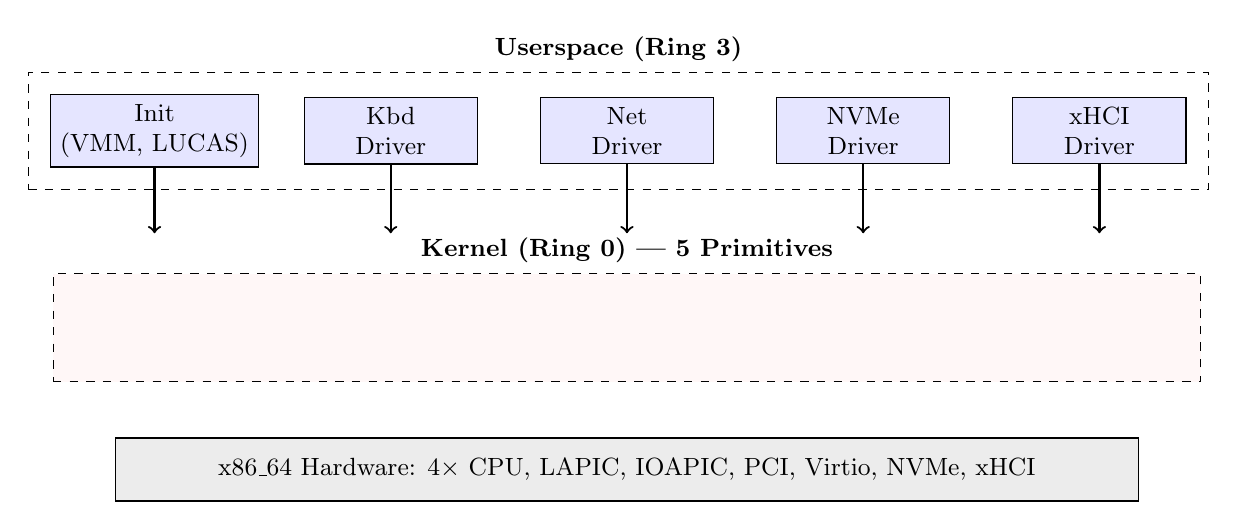
\begin{tikzpicture}[
    block/.style={rectangle, draw, fill=blue!10, minimum width=2.2cm, minimum height=0.8cm, align=center, font=\small},
    kblock/.style={rectangle, draw, fill=red!10, minimum width=2cm, minimum height=0.8cm, align=center, font=\small},
    arrow/.style={->, thick},
    every node/.style={font=\small}
]
    % Userspace
    \node[block] (init) at (0, 4) {Init\\(VMM, LUCAS)};
    \node[block] (kbd) at (3, 4) {Kbd\\Driver};
    \node[block] (net) at (6, 4) {Net\\Driver};
    \node[block] (nvme) at (9, 4) {NVMe\\Driver};
    \node[block] (xhci) at (12, 4) {xHCI\\Driver};

    % Userspace label
    \node[draw, dashed, fit=(init)(kbd)(net)(nvme)(xhci),
          inner sep=8pt, label=above:{\textbf{Userspace (Ring 3)}}] {};

    % Kernel
    \node[kblock] (sched) at (0, 1.5) {Scheduler};
    \node[kblock] (ipc) at (3, 1.5) {IPC};
    \node[kblock] (cap) at (6, 1.5) {Caps};
    \node[kblock] (irq) at (9, 1.5) {IRQ};
    \node[kblock] (frame) at (12, 1.5) {Frames};

    % Kernel label
    \node[draw, dashed, fill=red!3, fit=(sched)(ipc)(cap)(irq)(frame),
          inner sep=8pt, label=above:{\textbf{Kernel (Ring 0) --- 5 Primitives}}] {};

    % Hardware
    \node[rectangle, draw, fill=gray!15, minimum width=13cm, minimum height=0.8cm]
        (hw) at (6, -0.3) {x86\_64 Hardware: 4$\times$ CPU, LAPIC, IOAPIC, PCI, Virtio, NVMe, xHCI};

    % Arrows
    \draw[arrow] (init) -- ++(0,-1.3);
    \draw[arrow] (kbd) -- ++(0,-1.3);
    \draw[arrow] (net) -- ++(0,-1.3);
    \draw[arrow] (nvme) -- ++(0,-1.3);
    \draw[arrow] (xhci) -- ++(0,-1.3);
\end{tikzpicture}
\caption{sotOS architecture: five kernel primitives, all drivers in userspace.}
\label{fig:arch}
\end{figure}

The kernel implements exactly five primitives:

\begin{definition}[Kernel Primitives]
The sotOS kernel provides:
\begin{enumerate}[nosep]
    \item \textbf{Scheduling}: Preemptive priority multi-level queue with
          per-core run queues and work stealing.
    \item \textbf{IRQ Virtualization}: Hardware interrupts routed to userspace
          via notification objects.
    \item \textbf{IPC}: Per-core synchronous endpoints (L4-style register
          transfer) and async bounded channels.
    \item \textbf{Capability Management}: Generation-checked capability table
          with delegation tree and O(n) revocation.
    \item \textbf{Frame Allocation}: Bitmap-based physical frame allocator
          with contiguous allocation support.
\end{enumerate}
\end{definition}

% ============================================================================
\section{Per-Core IPC Architecture}
\label{sec:ipc}
% ============================================================================

\subsection{Motivation}

Traditional microkernels protect IPC state with a single global lock. On
multicore systems, this creates a serialization bottleneck: all cores contend
on the same lock for every IPC operation.

\begin{figure}[h]
\centering
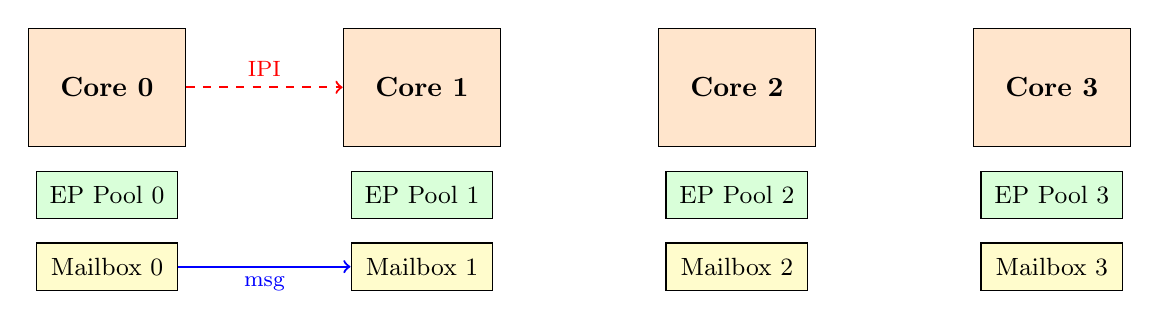
\begin{tikzpicture}[
    core/.style={rectangle, draw, fill=orange!20, minimum width=2cm, minimum height=1.5cm, align=center},
    pool/.style={rectangle, draw, fill=green!15, minimum width=1.8cm, minimum height=0.6cm, align=center, font=\small},
    mbox/.style={rectangle, draw, fill=yellow!20, minimum width=1.8cm, minimum height=0.6cm, align=center, font=\small},
    arrow/.style={->, thick, blue},
    ipi/.style={->, thick, red, dashed}
]
    \node[core] (c0) at (0,0) {\textbf{Core 0}};
    \node[core] (c1) at (4,0) {\textbf{Core 1}};
    \node[core] (c2) at (8,0) {\textbf{Core 2}};
    \node[core] (c3) at (12,0) {\textbf{Core 3}};

    \node[pool, below=0.3cm of c0] (p0) {EP Pool 0};
    \node[pool, below=0.3cm of c1] (p1) {EP Pool 1};
    \node[pool, below=0.3cm of c2] (p2) {EP Pool 2};
    \node[pool, below=0.3cm of c3] (p3) {EP Pool 3};

    \node[mbox, below=0.3cm of p0] (m0) {Mailbox 0};
    \node[mbox, below=0.3cm of p1] (m1) {Mailbox 1};
    \node[mbox, below=0.3cm of p2] (m2) {Mailbox 2};
    \node[mbox, below=0.3cm of p3] (m3) {Mailbox 3};

    % Cross-core IPC via mailbox + IPI
    \draw[ipi] (c0.east) -- node[above, font=\footnotesize] {IPI} (c1.west);
    \draw[arrow] (m0.east) -- node[below, font=\footnotesize] {msg} (m1.west);
\end{tikzpicture}
\caption{Per-core IPC: each core has its own endpoint pool and mailbox.
Cross-core delivery uses the mailbox queue + IPI for immediate wake.}
\label{fig:percore-ipc}
\end{figure}

\subsection{Handle Encoding}

Endpoint handles encode the owning core in the upper 4 bits:

\begin{equation}
\text{handle} = (\text{core\_id} \ll 28) \,|\, (\text{generation} \ll 20) \,|\, \text{slot\_index}
\end{equation}

This gives us 16 cores $\times$ 256 generations $\times$ 1M slots per core,
fitting in a single 32-bit value compatible with the capability system.

\subsection{Cross-Core Protocol}

\begin{algorithm}[h]
\caption{Per-Core IPC Send}
\begin{algorithmic}[1]
\Procedure{Send}{$\text{ep\_handle}, \text{msg}$}
    \State $(\text{core}, \text{local}) \gets \Call{Decode}{\text{ep\_handle}}$
    \If{$\text{core} = \text{my\_core}$}
        \Comment{Fast path: local lock only}
        \State \Call{LocalSend}{$\text{local}, \text{msg}$}
    \Else
        \Comment{Cross-core: lock target core's pool}
        \State \textbf{lock} $\text{PER\_CORE\_ENDPOINTS}[\text{core}]$
        \State $\text{action} \gets \Call{InspectEndpoint}{\text{local}}$
        \State \textbf{unlock}
        \State \Call{Execute}{$\text{action}$}
        \If{$\text{action requires wake on remote core}$}
            \State \Call{PostMailbox}{$\text{core}, \text{wake\_request}$}
            \State \Call{SendIPI}{$\text{core}$}
        \EndIf
    \EndIf
\EndProcedure
\end{algorithmic}
\end{algorithm}

\begin{theorem}[IPC Contention Reduction]
With $C$ cores and $N$ endpoints distributed uniformly, the expected lock
contention per IPC operation is $O(1/C)$ compared to $O(1)$ with a global
lock.
\end{theorem}

\begin{proof}
Each core's endpoint pool has its own lock. An IPC operation locks only the
target core's pool. With uniform distribution, each pool serves $N/C$
endpoints. The probability that two concurrent operations target the same
core's pool is $1/C$, reducing contention by a factor of $C$.
\end{proof}

% ============================================================================
\section{WASM Software Fault Isolation}
\label{sec:wasm}
% ============================================================================

\subsection{Design}

Traditional microkernels use hardware page tables for process isolation. This
requires TLB flushes on context switches and adds latency to IPC. Software
Fault Isolation (SFI) via WebAssembly provides an alternative: services are
compiled to WASM bytecode and executed by an interpreter that enforces memory
safety through bounds checking on every memory access.

\begin{figure}[h]
\centering
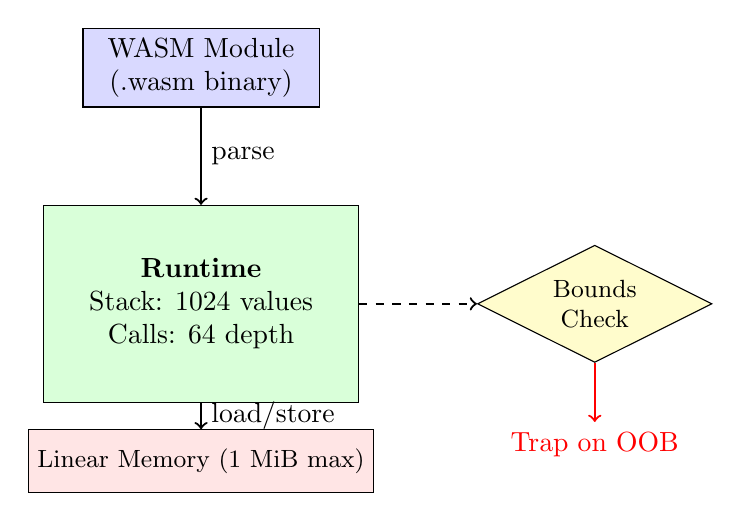
\begin{tikzpicture}[
    module/.style={rectangle, draw, fill=blue!15, minimum width=3cm, minimum height=1cm, align=center},
    rt/.style={rectangle, draw, fill=green!15, minimum width=4cm, minimum height=2.5cm, align=center},
    mem/.style={rectangle, draw, fill=red!10, minimum width=3.5cm, minimum height=0.8cm, align=center, font=\small},
    check/.style={diamond, draw, fill=yellow!20, aspect=2, align=center, font=\small}
]
    \node[module] (mod) at (0,3) {WASM Module\\(.wasm binary)};
    \node[rt] (rt) at (0,0) {\textbf{Runtime}\\Stack: 1024 values\\Calls: 64 depth};
    \node[mem] (mem) at (0,-2) {Linear Memory (1 MiB max)};
    \node[check] (chk) at (5,0) {Bounds\\Check};

    \draw[->, thick] (mod) -- node[right] {parse} (rt);
    \draw[->, thick] (rt) -- node[right] {load/store} (mem);
    \draw[->, thick, dashed] (rt) -- (chk);
    \draw[->, thick, red] (chk) -- ++(0,-1.5) node[below] {Trap on OOB};
\end{tikzpicture}
\caption{WASM SFI: every memory access goes through a bounds check.
Out-of-bounds accesses trap immediately without corrupting other memory.}
\label{fig:wasm-sfi}
\end{figure}

\subsection{Implementation}

The sotOS WASM runtime (\texttt{libs/sotos-wasm/}) is a \texttt{no\_std}
stack-based interpreter supporting:

\begin{itemize}[nosep]
    \item \textbf{Types}: \texttt{i32}, \texttt{i64} (integer arithmetic)
    \item \textbf{Operations}: 50+ opcodes including arithmetic, comparison,
          bitwise, memory load/store, control flow
    \item \textbf{Control flow}: \texttt{block}, \texttt{loop},
          \texttt{if/else}, \texttt{br}, \texttt{br\_if}, \texttt{return},
          \texttt{call}
    \item \textbf{Memory}: Linear memory with configurable size (up to 1 MiB),
          bounds-checked on every access
    \item \textbf{Module format}: Full WASM binary parser (magic, version,
          type/function/memory/global/export/code sections)
\end{itemize}

\begin{invariant}[Memory Safety]
For all memory operations $\texttt{load}(a, s)$ and $\texttt{store}(a, s, v)$
where $a$ is the address and $s$ is the access size:
\[
a + s \leq |\text{memory}| \quad \text{or the operation traps.}
\]
No memory access can read or write outside the module's linear memory region.
\end{invariant}

\subsection{Comparison with Hardware Isolation}

\begin{table}[h]
\centering
\begin{tabular}{lcc}
\toprule
\textbf{Property} & \textbf{Page Tables} & \textbf{WASM SFI} \\
\midrule
Context switch cost & TLB flush ($\sim$1000 cycles) & None (same address space) \\
IPC overhead & CR3 switch + sysret & Direct function call \\
Memory granularity & 4 KiB pages & 1 byte \\
Isolation guarantee & Hardware-enforced & Software-enforced \\
TCB size & CPU microcode + kernel & WASM interpreter ($\sim$1500 LOC) \\
\bottomrule
\end{tabular}
\caption{Comparison of hardware vs.\ software fault isolation.}
\label{tab:isolation}
\end{table}

% ============================================================================
\section{Capability System}
\label{sec:caps}
% ============================================================================

\subsection{Design}

Every kernel object in sotOS is accessed through \emph{capabilities}:
unforgeable tokens that combine an object reference with a set of rights.
Capabilities are stored in a generation-checked pool, making stale references
detectable in O(1) time.

\begin{definition}[Capability]
A capability $c = (\text{object}, \text{rights}, \text{parent}, \text{gen})$
where:
\begin{itemize}[nosep]
    \item $\text{object}$ identifies a kernel object (endpoint, thread, frame, etc.)
    \item $\text{rights} \subseteq \{\texttt{R}, \texttt{W}, \texttt{X}, \texttt{G}, \texttt{V}\}$
    \item $\text{parent}$ links to the derivation tree for revocation
    \item $\text{gen}$ is a generation counter for ABA protection
\end{itemize}
\end{definition}

\begin{theorem}[Monotonic Rights]
For any capability $c'$ derived from $c$ via $\text{Grant}(c, \text{mask})$:
\[
\text{rights}(c') = \text{rights}(c) \cap \text{mask} \subseteq \text{rights}(c)
\]
A derived capability never has more rights than its parent.
\end{theorem}

\begin{proof}
The $\text{Grant}$ operation computes $\text{rights}(c') = \text{rights}(c) \wedge \text{mask}$
(bitwise AND). Since $A \wedge B \subseteq A$ for all bitsets $A, B$, the
derived rights are always a subset.
\end{proof}

\subsection{Capability Derivation Tree}

\begin{figure}[h]
\centering
\begin{tikzpicture}[
    cap/.style={circle, draw, fill=blue!15, minimum size=1cm, align=center, font=\small},
    dead/.style={circle, draw, fill=red!30, minimum size=1cm, align=center, font=\small},
    level 1/.style={sibling distance=3.5cm},
    level 2/.style={sibling distance=2cm}
]
    \node[cap] {RWG}
        child { node[cap] {RW}
            child { node[cap] {R} }
            child { node[cap] {W} }
        }
        child { node[cap] {RG}
            child { node[cap] {R} }
        };
\end{tikzpicture}
\caption{Capability Derivation Tree. Each node shows the rights of that
capability. Revoking the root invalidates the entire subtree.}
\label{fig:cdt}
\end{figure}

% ============================================================================
\section{Scheduler}
\label{sec:sched}
% ============================================================================

\subsection{Multi-Level Priority Queue}

The scheduler uses a 4-level priority queue per CPU core:

\begin{table}[h]
\centering
\begin{tabular}{clc}
\toprule
\textbf{Level} & \textbf{Name} & \textbf{Priority Range} \\
\midrule
0 & Realtime & 0--63 \\
1 & High & 64--127 \\
2 & Normal & 128--191 \\
3 & Low & 192--255 \\
\bottomrule
\end{tabular}
\caption{Priority classes in the multi-level feedback queue.}
\label{tab:priority}
\end{table}

\subsection{Work Stealing}

When a CPU's run queue is empty, it steals the lowest-priority thread from
another CPU's queue. This ensures load balancing without centralized
coordination:

\begin{algorithm}[h]
\caption{Work Stealing}
\begin{algorithmic}[1]
\Procedure{DequeueFromAny}{$\text{my\_cpu}$}
    \If{$\text{PER\_CPU\_QUEUES}[\text{my\_cpu}].\text{pop\_front}() \neq \bot$}
        \State \Return thread \Comment{Fast path: local queue}
    \EndIf
    \For{$\text{offset} \gets 1$ \textbf{to} $C-1$}
        \State $\text{victim} \gets (\text{my\_cpu} + \text{offset}) \bmod C$
        \If{$\text{try\_lock}(\text{victim})$ succeeds}
            \If{$\text{PER\_CPU\_QUEUES}[\text{victim}].\text{pop\_back\_lowest}() \neq \bot$}
                \State \Return stolen\_thread
            \EndIf
        \EndIf
    \EndFor
    \State \Return $\bot$ \Comment{No work available}
\EndProcedure
\end{algorithmic}
\end{algorithm}

\subsection{Heterogeneous Compute Targets}

Threads are tagged with a \texttt{ComputeTarget} indicating whether they
should execute on CPU, GPU, or NPU hardware:

\begin{equation}
\text{ComputeTarget} \in \{\texttt{CPU}, \texttt{GPU}, \texttt{NPU}\}
\end{equation}

The scheduler filters dequeued threads by compute target, ensuring that
GPU/NPU workloads are not scheduled on CPU cores but instead queued for
offload to the appropriate accelerator.

% ============================================================================
\section{Network-Transparent IPC}
\label{sec:swarm}
% ============================================================================

The IPC routing layer extends endpoint addressing with a 16-bit node ID,
enabling transparent message delivery across a network of sotOS nodes:

\begin{figure}[h]
\centering
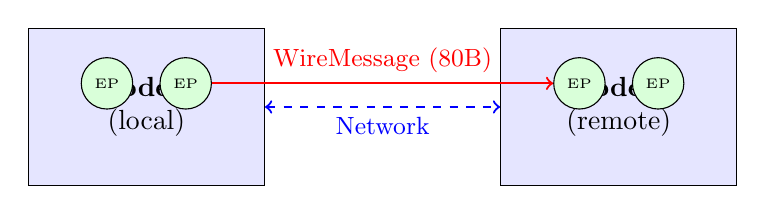
\begin{tikzpicture}[
    node/.style={rectangle, draw, fill=blue!10, minimum width=3cm, minimum height=2cm, align=center},
    ep/.style={circle, draw, fill=green!15, minimum size=0.6cm, font=\tiny}
]
    \node[node] (n0) at (0,0) {\textbf{Node 0}\\(local)};
    \node[node] (n1) at (6,0) {\textbf{Node 1}\\(remote)};

    \node[ep] (e0) at (-0.5, 0.3) {EP};
    \node[ep] (e1) at (0.5, 0.3) {EP};
    \node[ep] (e2) at (5.5, 0.3) {EP};
    \node[ep] (e3) at (6.5, 0.3) {EP};

    \draw[->, thick, red] (e1) -- node[above, font=\small] {WireMessage (80B)} (e2);
    \draw[<->, thick, dashed, blue] (n0.east) -- node[below, font=\small] {Network} (n1.west);
\end{tikzpicture}
\caption{Network-transparent IPC: messages to remote endpoints are
serialized to a fixed 80-byte wire format and routed over the network.}
\label{fig:swarm}
\end{figure}

Messages are serialized using a fixed-size \texttt{WireMessage} format (80
bytes), which includes the tag, 8 register values, capability transfer ID, and
flags. The routing table maps local proxy endpoints to remote
(node\_id, endpoint\_handle) pairs.

% ============================================================================
\section{Formal Verification}
\label{sec:formal}
% ============================================================================

We provide TLA+ specifications for three core protocols:

\subsection{IPC Protocol (formal/ipc.tla)}

The IPC specification models the synchronous rendezvous protocol with
\texttt{Send}, \texttt{Recv}, and \texttt{Call} operations. We verify:

\begin{invariant}[No Double Delivery]
No message is delivered to two different receivers:
\[
\forall d_1, d_2 \in \text{delivered}: d_1 = d_2 \lor d_1.\text{sender} \neq d_2.\text{sender} \lor d_1.\text{receiver} \neq d_2.\text{receiver}
\]
\end{invariant}

\begin{invariant}[Single Receiver]
At most one thread can be waiting to receive on an endpoint at any time:
\[
\text{state} = \texttt{recv\_wait} \implies \text{receiver} \neq \texttt{NULL}
\]
\end{invariant}

\subsection{Capability System (formal/capabilities.tla)}

The capability specification verifies:
\begin{itemize}[nosep]
    \item \textbf{No Unauthorized Access}: Every access uses a valid, alive
          capability with the required right.
    \item \textbf{Monotonic Rights}: Derived capabilities never exceed parent
          rights.
    \item \textbf{Revocation Completeness}: Dead capabilities have dead
          descendants.
\end{itemize}

\subsection{Scheduler (formal/scheduler.tla)}

The scheduler specification verifies:
\begin{itemize}[nosep]
    \item \textbf{Mutual Exclusion}: Each CPU runs at most one thread.
    \item \textbf{Single Execution}: No thread runs on two CPUs simultaneously.
    \item \textbf{No Starvation}: Under weak fairness, every ready thread
          eventually runs.
\end{itemize}

% ============================================================================
\section{Security Architecture}
\label{sec:security}
% ============================================================================

sotOS implements defense-in-depth security:

\begin{enumerate}[nosep]
    \item \textbf{W\^{}X Enforcement}: Pages cannot be both writable and
          executable. The kernel automatically adds the NX bit to writable
          mappings. A \texttt{SYS\_PROTECT} syscall allows changing permissions
          post-mapping with W\^{}X enforced.
    \item \textbf{Stack Guard Pages}: An unmapped page below each process
          stack triggers a page fault on stack overflow.
    \item \textbf{ASLR}: Stack base addresses are randomized using a
          RDTSC-seeded xorshift64 PRNG with 0--64~KiB jitter.
    \item \textbf{Stack Canaries}: Built with \texttt{-Z stack-protector=strong},
          providing $\sim$1800 canary check sites per binary.
    \item \textbf{Capability Isolation}: Processes can only access kernel
          objects through explicitly granted capabilities.
\end{enumerate}

% ============================================================================
\section{Storage Architecture}
\label{sec:storage}
% ============================================================================

The file system is built on a transactional object store with write-ahead
logging (WAL) for crash recovery:

\begin{figure}[h]
\centering
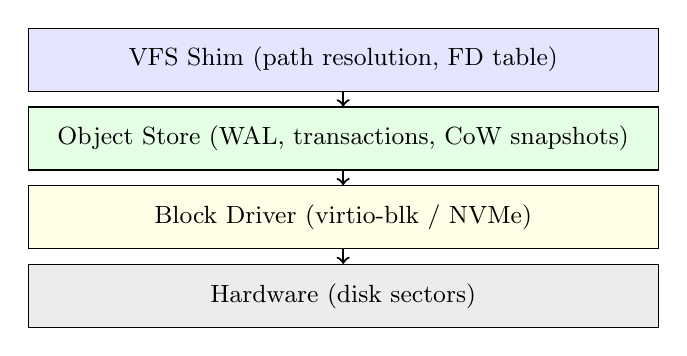
\begin{tikzpicture}[
    layer/.style={rectangle, draw, minimum width=8cm, minimum height=0.8cm, align=center, font=\small},
]
    \node[layer, fill=blue!10] (vfs) at (0, 3) {VFS Shim (path resolution, FD table)};
    \node[layer, fill=green!10] (obj) at (0, 2) {Object Store (WAL, transactions, CoW snapshots)};
    \node[layer, fill=yellow!10] (drv) at (0, 1) {Block Driver (virtio-blk / NVMe)};
    \node[layer, fill=gray!15] (hw) at (0, 0) {Hardware (disk sectors)};

    \draw[->, thick] (vfs) -- (obj);
    \draw[->, thick] (obj) -- (drv);
    \draw[->, thick] (drv) -- (hw);
\end{tikzpicture}
\caption{Storage stack: VFS $\to$ Object Store $\to$ Block Driver $\to$ Hardware.}
\label{fig:storage}
\end{figure}

Features include:
\begin{itemize}[nosep]
    \item Large file support (streaming I/O, 512~KiB max)
    \item Directory hierarchy with parent tracking
    \item Copy-on-Write snapshots with reference-counted blocks
    \item File permissions and ownership (UNIX-style rwx model)
\end{itemize}

% ============================================================================
\section{Networking}
\label{sec:net}
% ============================================================================

The networking stack (\texttt{libs/sotos-net/}) implements a full IP stack:

\begin{itemize}[nosep]
    \item Ethernet + ARP (32-entry cache)
    \item IPv4 with ICMP echo (ping)
    \item UDP (16 sockets) with DNS resolution
    \item TCP (16 connections, 3-way handshake, retransmission with
          exponential backoff)
    \item DHCP client for automatic configuration
\end{itemize}

The network driver runs in a separate userspace process with its own address
space, communicating with the shell via IPC.

% ============================================================================
\section{Implementation Statistics}
\label{sec:stats}
% ============================================================================

\begin{table}[h]
\centering
\begin{tabular}{lr}
\toprule
\textbf{Component} & \textbf{Lines of Rust} \\
\midrule
Kernel & $\sim$4,500 \\
sotos-common (ABI) & $\sim$800 \\
sotos-wasm (interpreter) & $\sim$1,200 \\
sotos-net (TCP/IP stack) & $\sim$2,000 \\
sotos-objstore (filesystem) & $\sim$1,500 \\
sotos-nvme (NVMe driver) & $\sim$800 \\
sotos-xhci (USB driver) & $\sim$1,300 \\
Services (init, shell, etc.) & $\sim$5,000 \\
\midrule
\textbf{Total} & $\sim$17,100 \\
\bottomrule
\end{tabular}
\caption{Approximate lines of code by component.}
\label{tab:loc}
\end{table}

\begin{table}[h]
\centering
\begin{tabular}{lr}
\toprule
\textbf{Feature} & \textbf{Count} \\
\midrule
Syscall numbers defined & 42 \\
Capability object types & 10 \\
Userspace processes & 8 \\
Device drivers & 5 \\
Shell builtins & 25+ \\
WASM opcodes supported & 50+ \\
TLA+ specifications & 3 \\
Stack canary check sites & $\sim$1,800/binary \\
\bottomrule
\end{tabular}
\caption{Feature counts.}
\label{tab:features}
\end{table}

% ============================================================================
\section{Conclusion}
% ============================================================================

sotOS demonstrates that a formally-verifiable microkernel can combine the
safety of capability-based security with the performance of per-core
architecture. The per-core IPC design reduces lock contention by $C\times$ on
$C$-core systems. The WASM runtime provides an alternative isolation mechanism
that eliminates TLB flush overhead. And the TLA+ specifications provide a
foundation for machine-checked correctness proofs.

Future work includes:
\begin{itemize}[nosep]
    \item Connecting the WASM runtime to the service loading pipeline
    \item Implementing the network transport for distributed IPC
    \item Live process migration between nodes
    \item GPU/NPU driver integration for heterogeneous scheduling
    \item Mechanized proofs using Coq or Lean for the verified kernel subset
\end{itemize}

\end{document}
